\section{Resource Manager Configuration: Classes and Nodepools}
\label{sec:ducc.classes}

The class configuration file is used by the Resource Manager configures the rules used for job
scheduling. See the \hyperref[chap:rm]{Resource Manager chapter} for a detailed description of the DUCC
scheduler, scheduling classes, and how classes are used to configure the scheduling process.

The scheduler  configuration file is specified in ducc.properties. The default name is 
ducc.classes and is specified by the property {\em ducc.rm.class.definitions}.
  
\subsection{Nodepools}
\label{subsec:nodepools}

\subsubsection{Overview}
    A {\em nodepool} is a grouping of a subset of the physical nodes to allow differing
    scheduling policies to be applied to different nodes in the system.  Some typical
    nodepool groupings might include:
    \begin{enumerate}
      \item Group Intel and Power nodes separately so that users may submit jobs that run
        only in Intel architecture, or only Power, or ``don't care''.
      \item Designate a group of nodes with large locally attached disks such that users
        can run jobs that require those disks.
      \item Designate a specific set of nodes with specialized hardware such as high-speed
        network, such that jobs can be scheduled to run only on those nodes.
    \end{enumerate}

    A Nodepool is a subset of some larger collection of nodes.  Nodepools themselves may be
    further subdivided.  Nodepools may not overlap: every node belongs to exactly
    one nodepool.  During system start-up the consistency of nodepool definition is checked
    and the system will refuse to start if the configuration is incorrect.

    For example, the diagram below is an abstract representation of all the nodes in a
    system.  There are five nodepools defined:
    \begin{itemize}
      \item Nodepool ``NpAllOfThem'' is subdivided into three pools, NP1, NP2, and NP3.  All
        the nodes not contained in NP1, NP2, and NP3 belong to the pool called ``NpAllOfThem''.
      \item Nodepool NP1 is not further subdivided.
      \item Nodepool NP2 is not further subdivided.
      \item Nodepool NP3 is further subdivided to form NP4.  All nodes within NP3 but
        not in NP4 are contained in NP3.
      \item Nodepool NP4 is not further subdivided.
    \end{itemize}

    \begin{figure}[H]
      \centering
      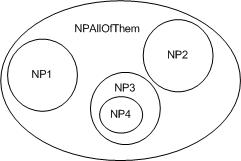
\includegraphics[bb=0 0 241 161, width=5.5in]{images/Nodepool1.jpg}
      \caption{Nodepool Example}
      \label{fig:Nodepools1}
    \end{figure}

    In the figure below the Nodepools are incorrectly defined for two reasons:
    \begin{enumerate}
       \item NP1 and NP2 overlap.
       \item NP4 overlaps both nodepool ``NpAllOfThem'' and NP3.
    \end{enumerate}
    
    \begin{figure}[H]
      \centering
      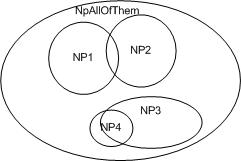
\includegraphics[bb=0 0 241 161, width=5.5in]{images/Nodepool2.jpg}
      \caption{Nodepools: Overlapping Pools are Incorrect}
      \label{fig:Nodepools2}
    \end{figure}

    Multiple ``top-level'' nodepools are allowed.  A ``top-level'' nodepool has no containing
    pool.  Multiple top-level pools logically divide a cluster of machines into {\em multiple
      independent clusters} from the standpoint of the scheduler.  Work scheduled over one
    pool in no way affects work scheduled over the other pool.  The figure below shows an
    abstract nodepool configuration with two top-level nodepools, ``Top-NP1'' and ``Top-NP2''.
    \begin{figure}[H]
      \centering
      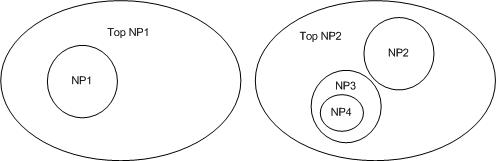
\includegraphics[bb=0 0 496 161, width=5.5in]{images/Nodepool3.jpg}
      \caption{Nodepools: Multiple top-level Nodepools}
      \label{fig:Nodepools3}
    \end{figure}

\subsubsection{Scheduling considerations}
    A primary goal of the scheduler is to insure that no resources are left idle if there
    is pending work that is able to use those resources.  Therefore, work scheduled to
    a class defined over a specific nodepool (say, NpAllOfThem), may be scheduled on nodes
    in any of the nodepools contained within NpAllOfThem.  If work defined over a
    subpool (such as NP1) arrives, processes on nodes in NP1 that were scheduled for
    NpAllOfThem are considered {\em squatters} and are the most likely candidates for
    eviction. (Processes assigned to their proper nodepools are considered {\em residents}
    and are evicted only after all {\em squatters} have been evicted.)  The scheduler strives
    to avoid creating {\em squatters}.

    Because non-preemptable allocations can't be preempeted, work submitted to a class
    implementing one of the non-preemptable policies (FIXED or RESERVE) are never allowed
    to ``squat'' in other nodepools and are only scheduled on nodes in their
    proper nodepool.

    In the case of multiple top-level nodepools: these nodepools and their sub-pools
    form independent scheduling groups.  Specifically,
    \begin{itemize}
        \item Fair-share allocations over any nodepool in one top-level pool do NOT affect the
          fair-share allocations for jobs in any other top-level nodepool. 

        \item Work submitted to classes under one top-level nodepool do NOT get expanded to
          nodes under another top-level nodepool, even is there is sufficient capacity.
    \end{itemize}

    Most installations will want to assign the majority of nodes to a single top-level
    nodepool (or its subpools), using other top-level pools for nodes that cannot be
    shared with other work.

\subsubsection{Configuration}
\label{subsubsec:nodepool.configuration}
    DUCC uses simple named stanzas containing key/value pairs to configure nodepools.

    At least one nodepool definition is required.  This nodepool need not have any subpools or node
    definitions.  The first top-level nodepool is considered the ``default'' nodepool.  Any node not
    named specifically in one of the node files which checks in with DUCC is assigned to this
    first, {\em default} nodepool. 

    Thus, if only one nodepool is defined with no other attributes, all nodes are
    assigned to that pool.

    A nodepool definition consists of the token ``Nodepool'' followed by the 
    name of the nodepool, followed by a block delimited with ``curly'' braces \{ and \}.  This
    block contains the attributes of the nodepool as key/value pairs.
    Lineneds are ignored.  A semicolon ``$;$'' may optionally be used to
    delimit key/value pairs for readability, and an equals sign ``='' may optionally
    be used to delimit keys from values, also just for readability.  See the 
    \hyperref[fig:nodepool.configuration]{below}.

    The attributes of a Nodepool are:
    \begin{description}
      \item[domain] This is valid only in the ``default'' (first) nodepool.  Any node
        in any nodefile which does not have a domain, and any node which checks
        in to the Resource Manager without a domain name is assigned this domain name
        in order that the scheduler may deal entirely with full-qualified node names.

        If no {\em domain} is specified, DUCC will attempt to guess the domain based
        on the domain name returned on the node where the Resource Manager resides.

      \item[nodefile] This is the name of a file containing the names of the nodes
        which are members of this nodepool.

      \item[parent] This is used to indicate which nodepool is the logical parent.
        Any nodepool without a {\em parent} is considered a top-level nodepool.
    \end{description}
        
    The following example defines six nodepools, 
    \begin{enumerate}
      \item A top-level nodepool called ``--default--''.  All nodes not named
        in any nodefile are assigned to this nodepool.
      \item A top-level nodepool called ``jobdriver'', consisting of the nodes
        named in the file {\em jobdriver.nodes}.
      \item A subpool of ``--default--'' called ``intel'', consisting of the
        nodes named in {\em intel.nodes}.
      \item A subpool of ``--default--'' called ``power'', consisting of the
        nodes named in the file {\em power.nodes}.
      \item A subpool of ``intel'' called ``nightly-test'', consisting of the 
        nodes named in {\em nightly-test.nodes}.
      \item And a subpool of ``power'' called ``testing-p7'', consisting of the
        nodes named in {\em timing-ps.nodes}.
    \end{enumerate}

    \begin{figure}[H]
    
\begin{verbatim}
    Nodepool --default--  { domain bluej.net }
    Nodepool jobdriver    { nodefile jobdriver.nodes }
    
    Nodepool intel        { nodefile intel.nodes        ; parent --default-- }
    Nodepool power        { nodefile power.nodes        ; parent --default-- }

    Nodepool nightly-test { nodefile nightly-test.nodes ; parent intel }
    Nodepool timing-p7    { nodefile timing-p7.nodes    ; parent power }
\end{verbatim}
      \caption{Sample Nodepool Configuration}
      \label{fig:nodepool.configuration}

    \end{figure}    


    \subsection{Class Definitions}
    \label{subsubsec:class.configuration}

    Scheduler classes are defined in the same simple block language as
    nodepools.

    A simple inheritance (or ``template'') scheme is supported for classes.  Any
    class may be configured to ``derive'' from any other class.  In this case, the
    child class acquires all the attributes of the parent class, any of which may
    be selectively overridden.  Multiple inheritance is not supported but
    nested inheritance is; that is, class A may inherit from class B which inherits
    from class C and so on. In this way, generalized templates for the site's
    class structure may be defined.  

    The general form of a class definition consists of the keyword Class, followed
    by the name of the class, and then optionally by the name of a ``parent'' class
    whose characteristics it inherits.   Following the name (and optionally parent class
    name) are the attributes of the class, also within a \{ block \} as for nodepools, and
    with lines and key/value pairs optionally delimited by  ``$;$'' and ``$=$'', respectively.
    See the sample \hyperref[fig:class.configuration]{below}.

    The attributes defined for classes are:
    \begin{description}

      \item[abstract] If specified, this indicates this class is a template ONLY. It is used
        as a model for other classes.  Values are ``true'' or ``false''.  The default is
        ``false''.  This class is never passed to the scheduler and may not be referenced
        by jobs.

      \item[cap] This specifies the largest number of shares that any job in this class
        may be assigned.  It may be an absolute number or a percentage.  If specified as
        a percentage (i.e. it contains a trailing \%), it specifies a percentage of the
        total nodes in the containing nodepool.

      \item[debug] FAIR\_SHARE only. This specifies the name of a class to substitute
        for jobs submitted for debug.  For example, if class {\em normal} specifies
\begin{verbatim}
     debug = fixed
\end{verbatim}
        then any job submitted to this class with debugging requested is actually scheduled
        in class {\em fixed}. (For example, one probably does not want a debugging job
        scheduled as FAIR\_SHARE and possibly preempted, preferring the non-preemptable
        class {\em fixed}.

      \item[default] This specifies the class to be used as the default class for work submission
        if no class is explicitly given.  Only one class of type FAIR\_SHARE may contain this
        designation, in which case it names the default FAIR\_SHARE class.  Only one class of type
        FIXED\_SHARE or RESERVE may contain this designation, in which case it names the default
        class to use for reservations (Note that either FIXED\_SHARE or RESERVE scheduling policies
        are valid for reservations.)

      \item[enforce] RESERVE only.  If specified, then reservations for this class must specify a
        memory size that exactly matches an eligible machine, modulo the share quanta.  For example,
        if the share quanta is 15G, a 15G reservation will never be honored on a 256G machine; in this
        case a 240G (or more) reservations must be specified.  The DUCC Web Server's {\em Machines} page
        displays the recommended request size for every machine.  

        If {\em enforce} is not specified, the default is ``true''.

        If {\em enforce} is set to false, the scheduler will attempt to match the reservation as 
        closely as possible to an existing machine, and if it cannot it will use the next largest
        machine available.  Thus, a 15G reservation {\em might} be satisfied with a 240G machine if
        that is all that is available at the time.

      \item[expand-by-doubling] FAIR\_SHARE only.  If ``true'', and the {\em initialization-cap} is
        set, then after any process has initialized, the job will expand to its maximum allowable
        shares by doubling in size each scheduling cycle.  

        If not specified, the global value set in \hyperref[sec:ducc.properties]{ducc.properties} is used.

      \item[initialization-cap] FAIR\_SHARE only. If specified, this is the largest number of processes this job
        may be assigned until at least one process has successfully completed initialization.

        If not specified, the global value set in \hyperref[sec:ducc.properties]{ducc.properties} is used.

      \item[max-processes] FAIR\_SHARE and FIXED\_SHARE only.  This is the largest number of FIXED-SHARE,
        non-preemptable shares any single job may be assigned.

        Omit this property, or set it to 0 to disable the cap.

      \item[max-machines] RESERVE only.  This specifies the maximum number of full machines that
        may be reserved by any single job.

        Omit this property, or set it to 0 to disable the cap.

      \item[prediction-fudge] FAIR\_SHARE only. When the scheduler is considering expanding the
        number of processes for a job it tries to determine if the job may complete before those
        processes are allocated and initialized.  The {\em prediction-fudge} adds some amount of 
        time (in milliseconds) to the projected completion time.  This allows installations to
        prevent jobs from expanding when they were otherwise going to end in a few minutes
        anyway.

        If not specified, the global value set in \hyperref[sec:ducc.properties]{ducc.properties} is used.

      \item[nodepool] If specified, jobs for this class are assigned to nodes in this nodepool. The
        value must be the name of one of the configured nodepools.

      \item[policy] This is the scheduling policy, one of FAIR\_SHARE, FIXED\_SHARE, or RESERVE. This
        attribute is required (there is no default).

      \item[priority] This is the scheduling priority for jobs in this class.

      \item[weight] FAIR\_SHARE only. This is the fair-share weight for jobs in this class.
      
    \end{description}

    The following figure illustrates a representative class configuration for a large cluster,
    consisting of mixed Intel and Power nodes.  This class definition assumes the
    \hyperref[fig:nodepool.configuration]{nodepool configuration} shown above.  FAIR\_SHARE,
    FIXED\_SHARE, and RESERVE classes are defined over each machine architecture, Intel and Power,
    and over the combined pool. 

    \begin{figure}[H]    
\begin{verbatim}
# --------------------- Fair share definitions ---------------
Class fair-base {
      policy = FAIR_SHARE
      nodepool = intel
      priority = 10
      weight = 100
      abstract = true
      debug = fixed
}

Class nightly-test   fair-base  { weight = 100; nodepool nightly-test; priority = 7}

Class background     fair-base  { weight = 20 }
Class low            fair-base  { weight = 50 }
Class normal         fair-base  { weight = 100; default = true }
Class high           fair-base  { weight = 200 }
Class weekly         fair-base  { weight = 400 }

Class background-p7  background { nodepool = power }
Class low-p7         low        { nodepool = power }
Class normal-p7      normal     { nodepool = power }
Class high-p7        high       { nodepool = power }
Class weekly-p7      weekly     { nodepool = power }

Class background-all background { nodepool = --default-- }
Class low-all        low        { nodepool = --default-- }
Class normal-all     normal     { nodepool = --default-- }
Class high-all       high       { nodepool = --default-- }
Class weekly-all     weekly     { nodepool = --default-- }

# --------------------- Fixed share definitions ---------------
Class fixed-base {
      policy = FIXED_SHARE
      nodepool = intel
      priority = 5
      abstract = true
      max-processes = 10
}

Class fixed     fixed-base { }
Class fixed-p7  fixed-base { nodepool = power;    default = true; }
Class JobDriver fixed-base { nodepool = jobdriver; priority = 0 }      

# --------------------- Reserve definitions ---------------
Class reserve-base {
      policy = RESERVE
      nodepool = intel
      priority = 1
      enforce = true
      abstract = true
      max-machines = 10
}
 
Class reserve     reserve-base { }
Class reserve-p7  reserve-base { nodepool = power }
Class timing-p7   reserve-base { nodepool = timing-p7 }
\end{verbatim}
          \caption{Sample Class Configuration}
      \label{fig:class.configuration}
    \end{figure}
    
\subsection{Validation}

The administrative command, \hyperref[subsec:admin.check-ducc]{\em check\_ducc} may be used to
validate a configuration, with the {\em -c} option.  This reads the entire configuration and
nodefiles, validates consistency of the definitions and insures the nodepools do not overlap.

During start-up, the \hyperref[subsec:admin.check-ducc]{\em start\_ducc} command always runs full validation, and if the
configuration is found to be incorrect, the cluster is not started.

Configuration checking is done internally by the DUCC java utility {\em
  org.apache.uima.ducc.commonNodeConfiguration}.  This utility contains a public
API as described in the Javadoc.  It may be invoked from the command line as follows:

    \paragraph{Usage:}
\begin{verbatim}
     java org.apache.uima.ducc.commonNodeConfiguration [-p] [-v nodefile] configfile
\end{verbatim}

    \paragraph{Options:}
    \begin{description}

      \item[$-p$] Pretty-print the compiled configuration to stdout. This illustrates
        nodepool nesting, and shows the fully-completed scheduling classes after inheritance.

      \item[$-v$ nodefile] This should be the master nodelist used to start DUCC.  This
        is assumed to be constructed to reflect the nodepool organization as 
        \hyperref[sec:admin-ducc.nodes]{described here}.  If provided,
        the nodepools are validated and checked for overlaps.

      \item[configfile] This is the name of the file containing the configuration.
    \end{description}
    
